%************************************************
\chapter{Analisi dei requisiti}\label{ch:requisiti}
%************************************************
Il seguente capitolo descrive le caratteristiche principali che l'azienda \myCompany richiede vengano implementate nel prototipo: dopo una descrizione generale vengono descritti i casi d'uso rilevati e i requisiti che ne derivano.

\section{Descrizione generale}
L'obiettivo dell'azienda è studiare le possibili implementazioni delle librerie esistenti (Sencha Touch e Cordova)per l'utilizzo dei sensori presenti nei device mobili con lo scopo di integrare tali caratteristiche in un prototipo dimostrativo funzionante su piattaforma Android e iOS.
Le funzionalità che risulteranno essere perfettamente funzionanti verranno integrate nell'applicativo che l'azienda sta sviluppando su richiesta di alcuni clienti.

Le funzionalità a cui l'azienda è interessata sono le seguenti:
\begin{itemize}
\item Scansione barcode;
\item Cattura immagini, video, registrazioni audio;
\item Lettura elenco contatti del dispositivo in uso;
\item Recupero informazioni proprie del dispositivo;
\item Backup e ripristino dei dati dell'applicazione sulla memoria di massa del dispositivo tramite un database \emph{SQLite}\footnote{\url{http://www.sqlite.org/}};
\item Geolocalizzazione.
\end{itemize}

Essendo tale applicazione un prototipo interno all'azienda non sono richiesti particolari vincoli di efficienza e un'interfaccia grafica accattivante: è stata lasciata libera iniziativa di sviluppare diverse soluzioni con l'obiettivo finale di ottenere un resoconto dettagliato dei risultati ottenuti.

\section{Casi d'uso}
Vengono ora descritti i casi d'uso utilizzati per la progettazione del prototipo richiesto.
Essi hanno un codice identificativo univoco, nella forma:
\begin{center}
UC[codice univoco del padre].[codice progressivo di livello]
\end{center}
Il codice progressivo di livello può includere diversi livelli di gerarchia separati da un punto.

\subsection{Caso d'uso UC1: Scenario principale}
\begin{figure}[htb]
\centering
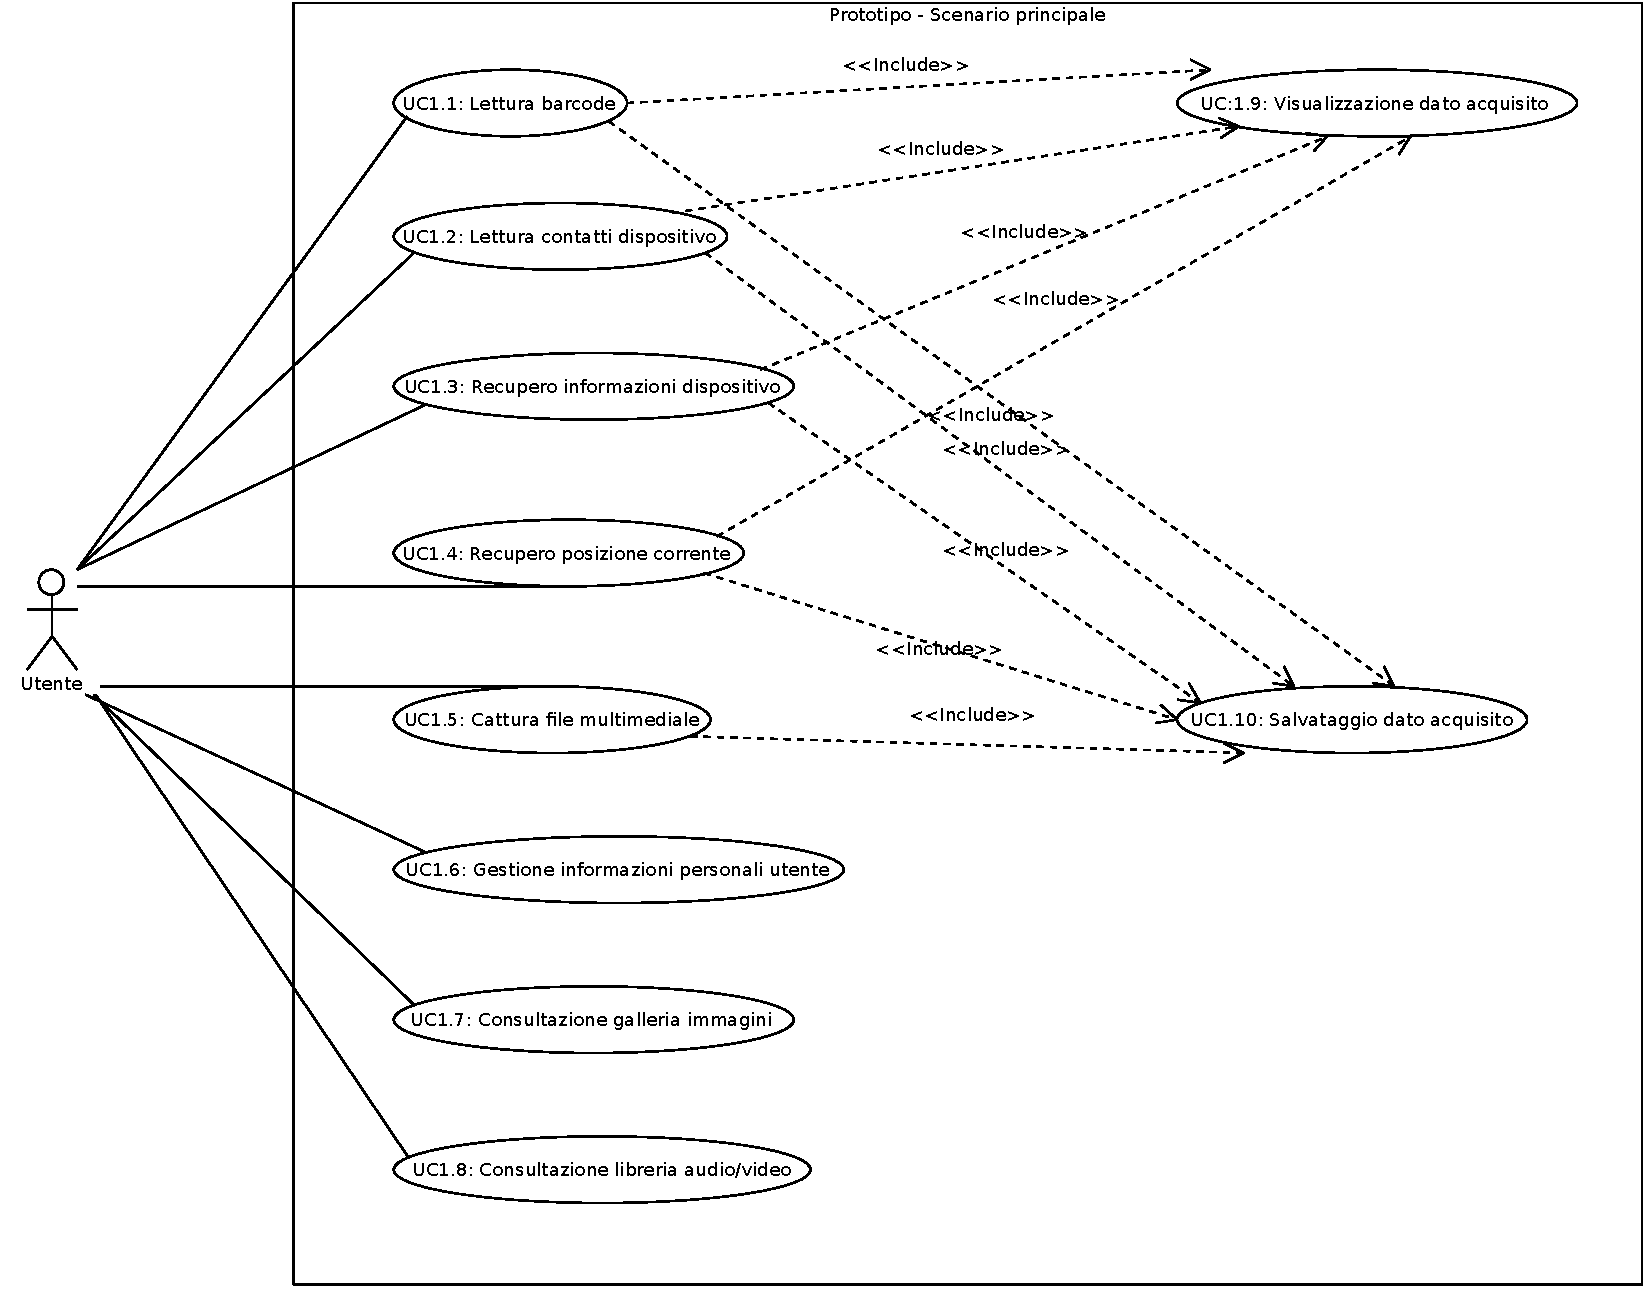
\includegraphics[scale=0.45]{gfx/useCase/UC1_Scenario_principale.pdf}
\caption{Caso d'uso UC1: Scenario principale}
\label{fig:UC1}
\end{figure}

\begin{description}
\item[attori:] Utente;
\item[scopo e descrizione:] L'utente ha avviato correttamente l'applicazione e questa è pronta all'uso. Egli può effettuare varie operazioni: leggere codici a barre, recuperare i contatti del dispositivo, recuperare le informazioni del dispositivo, catturare file multimediali, recuperare la posizione corrente dal \ac{GPS}, gestire le proprie informazioni personali, consultare la galleria immagini e la libreria audio/video, salvare e visualizzare i dati catturati tramite il dispositivo;
\item[precondizione:] L'applicazione è stata avviata ed è pronta all'uso.
\item[flusso principale degli eventi:] \hfill 
	\begin{enumerate}
	\item L'utente può leggere codici a barre;
	\item L'utente può recuperare i contatti del dispositivo;
	\item L'utente può recuperare le informazioni del dispositivo;
	\item L'utente può catturare file multimediali;
	\item L'utente può recuperare la posizione corrente;
	\item L'utente può gestire le proprie informazioni personali;
	\item L'utente può consultare la galleria;
	\item L'utente può consultare la libreria;
	\end{enumerate}
\item[inclusioni:] \hfill 
	\begin{enumerate}
	\item Il sistema salva i dati acquisiti;
	\item Il sistema visualizza i dati acquisiti;
	\end{enumerate}
\item[postcondizione:] Il sistema ha ottenuto informazioni sulle operazioni che l'utente vuole eseguire.
\end{description}

\subsection{Caso d'uso UC1.1: Lettura barcode}
\begin{description}
\item[attori:] Utente;
\item[scopo e descrizione:] L'utente ha scelto l'opzione di lettura di un codice a barre;
\item[precondizione:] Il sistema è pronto per la lettura di un nuovo codice;
\item[scenari alternativi:] \hfill 
	\begin{enumerate}
	\item L'utente decide di annullare l'operazione di lettura; il sistema torna allo stato precedente la scelta dell'utente;
	\end{enumerate}
\item[postcondizione:] Il sistema ha letto il codice e procede con il salvataggio e la visualizzazione dei dati.
\end{description}

\subsection{Caso d'uso UC1.2: Cattura file multimediale}
\begin{figure}[htb]
\centering
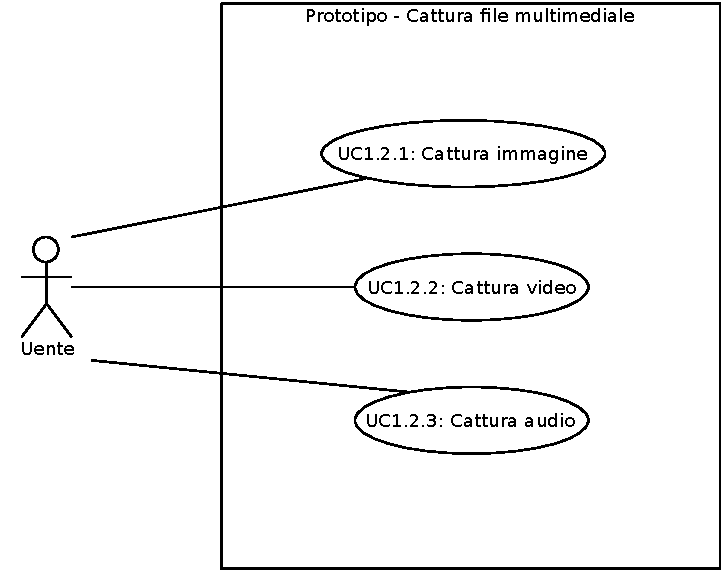
\includegraphics[scale=0.6]{gfx/useCase/UC1-2_Cattura_file_multimediale.pdf}
\caption{Caso d'uso UC1.2: Cattura file multimediale}
\label{fig:UC1.2}
\end{figure}

\begin{description}
\item[attori:] Utente;
\item[scopo e descrizione:] L'utente ha scelto l'opzione di cattura di un file multimediale e può decidere quale tipo di file catturare: immagine, audio o video;
\item[precondizione:] Il sistema mostra le possibili scelte all'utente;
\item[flusso principale degli eventi:] \hfill 
	\begin{enumerate}
	\item L'utente può catturare un'immagine;
	\item L'utente può catturare un video;
	\item L'utente può catturare un file audio;
	\end{enumerate}
\item[postcondizione:] Il sistema è pronto per la cattura del file multimediale prescelto.
\end{description}

\subsection{Caso d'uso UC1.2.1: Cattura immagine}
\begin{figure}[htb]
\centering
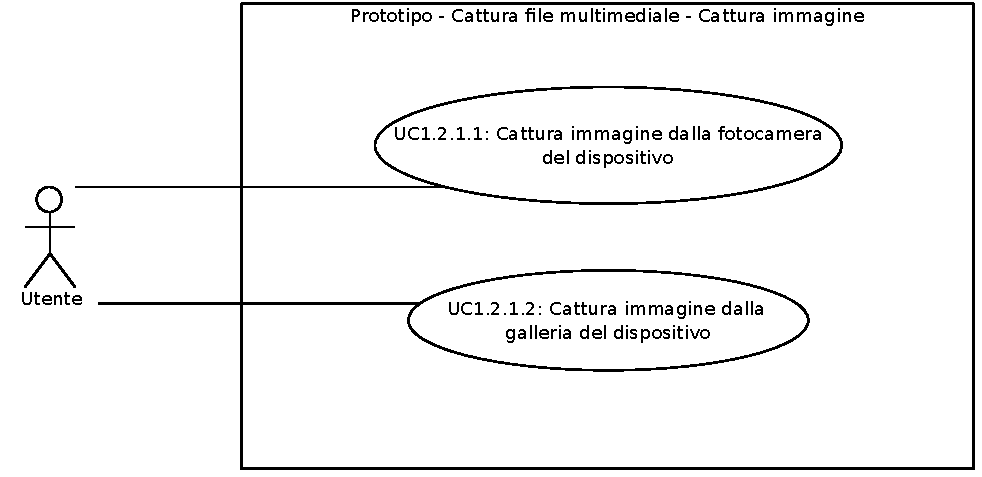
\includegraphics[scale=0.6]{gfx/useCase/UC1-2-1_Cattura_immagine.pdf}
\caption{Caso d'uso UC1.2.1: Cattura immagine}
\label{fig:UC1.2.1}
\end{figure}

\begin{description}
\item[attori:] Utente;
\item[scopo e descrizione:] L'utente ha scelto l'opzione di cattura di un'immagine e può scegliere se utilizzare la fotocamera del dispositivo oppure la galleria dello stesso;
\item[precondizione:] Il sistema mostra le possibili scelte all'utente;
\item[flusso principale degli eventi:] \hfill 
	\begin{enumerate}
	\item L'utente può catturare un'immagine dalla fotocamera del dispositivo;
	\item L'utente può catturare un'immagine dalla galleria del dispositivo;
	\end{enumerate}
\item[postcondizione:] Il sistema è pronto per la cattura dell'immagine dalla fonte prescelta.
\end{description}

\subsection{Caso d'uso UC1.2.1.1: Cattura immagine dalla fotocamera del dispositivo}
\begin{description}
\item[attori:] Utente;
\item[scopo e descrizione:] L'utente ha scelto la cattura di un'immagine dalla fotocamera del dispositivo;
\item[precondizione:] Il sistema è pronto per la cattura di una nuova immagine dalla fotocamera;
\item[scenari alternativi:] \hfill 
	\begin{enumerate}
	\item L'utente decide di annullare l'operazione di cattura; il sistema torna allo stato precedente la scelta dell'utente;
	\end{enumerate}
\item[postcondizione:] Il sistema ha catturato una nuova immagine e procede con il salvataggio.
\end{description}

\subsection{Caso d'uso UC1.2.1.2: Cattura immagine dalla galleria del dispositivo}
\begin{description}
\item[attori:] Utente;
\item[scopo e descrizione:] L'utente ha scelto la cattura di un'immagine dalla galleria del dispositivo;
\item[precondizione:] Il sistema è pronto per la cattura di una nuova immagine dalla galleria;
\item[scenari alternativi:] \hfill 
	\begin{enumerate}
	\item L'utente decide di annullare l'operazione di cattura; il sistema torna allo stato precedente la scelta dell'utente;
	\end{enumerate}
\item[postcondizione:] Il sistema ha catturato una nuova immagine e procede con il salvataggio.
\end{description}

\subsection{Caso d'uso UC1.2.2: Cattura video}
\begin{description}
\item[attori:] Utente;
\item[scopo e descrizione:] L'utente ha scelto la cattura di un video;
\item[precondizione:] Il sistema è pronto per la cattura di un nuovo video;
\item[scenari alternativi:] \hfill 
	\begin{enumerate}
	\item L'utente decide di annullare l'operazione di cattura; il sistema torna allo stato precedente la scelta dell'utente;
	\end{enumerate}
\item[postcondizione:] Il sistema ha catturato una nuovo video e procede con il salvataggio.
\end{description}

\subsection{Caso d'uso UC1.2.3: Cattura audio}
\begin{description}
\item[attori:] Utente;
\item[scopo e descrizione:] L'utente ha scelto la cattura di un file audio;
\item[precondizione:] Il sistema è pronto per la cattura di una nuovo file audio;
\item[scenari alternativi:] \hfill 
	\begin{enumerate}
	\item L'utente decide di annullare l'operazione di cattura; il sistema torna allo stato precedente la scelta dell'utente;
	\end{enumerate}
\item[postcondizione:] Il sistema ha catturato una nuovo file audio e procede con il salvataggio.
\end{description}

\subsection{Caso d'uso UC1.3: Recupero informazioni dispositivo}
\begin{description}
\item[attori:] Utente;
\item[scopo e descrizione:] L'utente ha scelto il recupero delle informazione del dispositivo;
\item[precondizione:] Il sistema è pronto per il recupero delle informazioni;
\item[postcondizione:] Il sistema ha recuperato le informazioni e procede con il salvataggio e la visualizzazione.
\end{description}

\subsection{Caso d'uso UC1.4: Recupero posizione corrente}
\begin{description}
\item[attori:] Utente,
\item[scopo e descrizione:] L'utente ha scelto il recupero della posizione corrente tramite il \ac{GPS} del dispositivo;
\item[precondizione:] Il sistema è pronto per il recupero della posizione;
\item[postcondizione:] Il sistema ha recuperato la posizione del dispositivo e procede con il salvataggio e la visualizzazione.
\end{description}

\subsection{Caso d'uso UC1.5: Lettura contatti dispositivo}
\begin{description}
\item[attori:] Utente;
\item[scopo e descrizione:] L'utente ha scelto la lettura dei contatti dal dispositivo;
\item[precondizione:] Il sistema è pronto per la lettura dei contatti presenti nel dispositivo;
\item[postcondizione:] Il sistema ha recuperato i contatti del dispositivo e procede con il salvataggio e la visualizzazione.
\end{description}

\subsection{Caso d'uso UC1.6: Gestione informazioni personali utente}
\begin{figure}[htb]
\centering
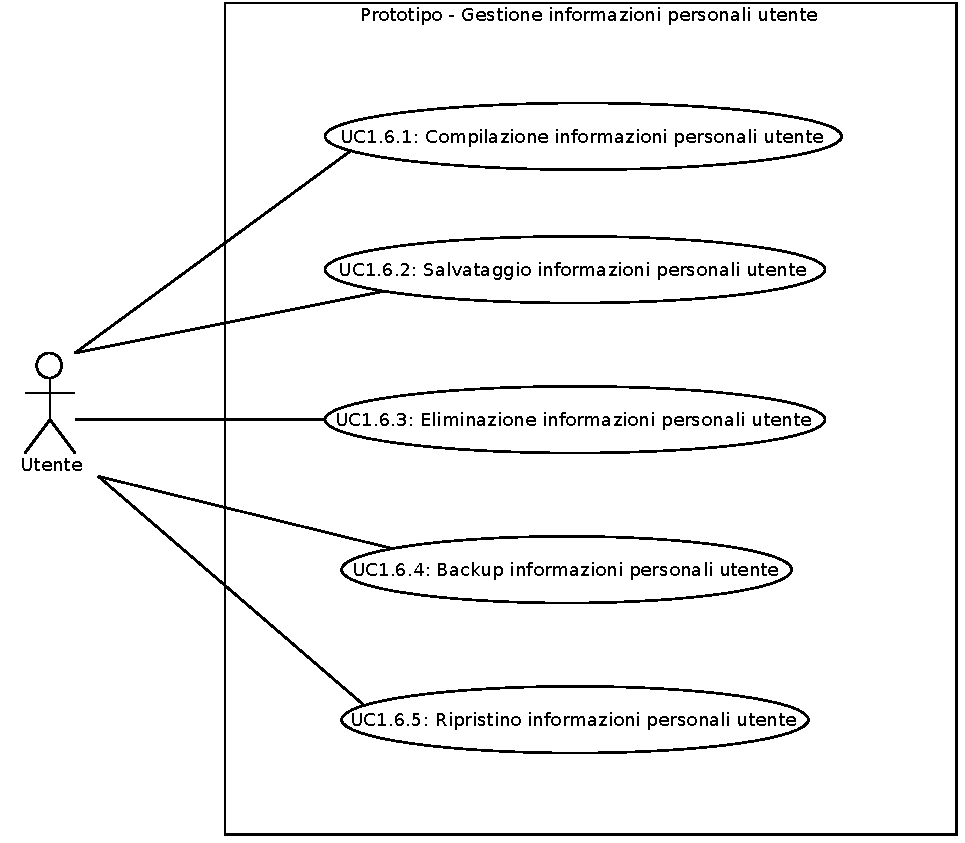
\includegraphics[scale=0.6]{gfx/useCase/UC1-6_Gestione_informazioni_personali_utente.pdf}
\caption{Caso d'uso UC1.6: Gestione informazioni personali utente}
\label{fig:UC1.6}
\end{figure}

\begin{description}
\item[attori:] Utente;
\item[scopo e descrizione:] L'utente ha scelto la gestione delle informazioni personali e può procedere con la compilazione di tali informazioni oppure salvare, eliminare, effettuare un backup o un ripristino di tali dati;
\item[precondizione:] Il sistema è pronto per gestire le informazioni personali dell'utente;
\item[flusso principale degli eventi:] \hfill
	\begin{enumerate}
	\item L'utente può compilare le informazioni personali;
	\item L'utente può salvare le informazioni personali;
	\item L'utente può eliminare le informazioni personali;
	\item L'utente può effettuare un backup delle informazioni personali;
	\item L'utente può effettuare un ripristino delle informazioni personali;
	\end{enumerate}
\item[postcondizione:] Il sistema è pronto ad eseguire l'opzione scelta dell'utente;
\end{description}

\subsection{Caso d'uso UC1.6.1: Compilazione informazioni personali utente}
\begin{description}
\item[attori:] Utente;
\item[scopo e descrizione:] L'utente ha scelto di compilare le informazioni personali;
\item[precondizione:] Il sistema è pronto per accettare l'immissione delle informazioni dell'utente;
\item[postcondizione:] Il sistema ha scritto le informazioni immesse dall'utente.
\end{description}

\subsection{Caso d'uso UC1.6.2: Salvataggio informazioni personali utente}
\begin{description}
\item[attori:] Utente;
\item[scopo e descrizione:] L'utente ha scelto di salvare le informazioni personali immesse;
\item[precondizione:] Il sistema è in possesso delle informazioni immesse dall'utente;
\item[postcondizione:] Il sistema ha salvato le informazioni immesse dall'utente.
\end{description}

\subsection{Caso d'uso UC1.6.3: Eliminazione informazioni personali utente}
\begin{description}
\item[attori:] Utente;
\item[scopo e descrizione:] L'utente ha scelto di eliminare le informazioni salvate;
\item[precondizione:] Il sistema possiede le informazioni dell'utente ed è pronto ad eliminarle;
\item[postcondizione:] Il sistema ha eliminato le informazioni dell'utente.
\end{description}

\subsection{Caso d'uso UC1.6.4: Backup informazioni personali utente}
\begin{description}
\item[attori:] Utente;
\item[scopo e descrizione:] L'utente ha scelto di effettuare un backup delle informazioni salvate;
\item[precondizione:] Il sistema possiede le informazioni salvate dell'utente ed è pronto al backup;
\item[postcondizione:] Il sistema ha effettuato il backup delle informazioni sulla memoria del dispositivo.
\end{description}

\subsection{Caso d'uso UC1.6.5: Ripristino informazioni personali utente}
\begin{description}
\item[attori:] Utente;
\item[scopo e descrizione:] L'utente ha scelto di ripristinare le informazioni di cui ha effettuato una copia di backup;
\item[precondizione:] Il sistema è pronto a ripristinare le informazioni dell'utente;
\item[postcondizione:] Il sistema a ripristinato le informazioni dell'utente.
\end{description}

\subsection{Caso d'uso UC1.7: Consultazione galleria immagini}
\begin{description}
\item[attori:] Utente;
\item[scopo e descrizione:] L'utente ha scelto di consultare la galleria delle immagini;
\item[precondizione:] Il sistema è pronto a visualizzare la galleria delle immagini;
\item[postcondizione:] Il sistema ha visualizzato la galleria delle immagini.
\end{description}

\subsection{Caso d'uso UC1.8: Consultazione libreria audio/video}
\begin{description}
\item[attori:] Utente;
\item[scopo e descrizione:] L'utente ha scelto di consultare la libreria audio/video;
\item[precondizione:] Il sistema è pronto a visualizzare la libreria audio/video;
\item[postcondizione:] Il sistema ha visualizzato la libreria audio/video.
\end{description}

\subsection{Caso d'uso UC1.9: Visualizzazione dato acquisito}
\begin{description}
\item[attori:] Sistema;
\item[scopo e descrizione:] Il sistema visualizza il dato acquisito;
\item[precondizione:] Il sistema è pronto a visualizzare il dato acquisito;
\item[postcondizione:] Il sistema ha visualizzato il dato acquisito.
\end{description}

\subsection{Caso d'uso UC1.10: Salvataggio dato acquisito}
\begin{description}
\item[attori:] Sistema;
\item[scopo e descrizione:] Il sistema salva il dato acquisito;
\item[precondizione:] Il sistema è pronto a visualizzare il dato acquisito;
\item[postcondizione:] Il sistema ha salvato il dato acquisito.
\end{description}

\newpage
\section{Requisiti}
Di seguito vengono riportati i requisiti individuati dall'analisi effettuata sulle richieste dell'azienda, emersi dai casi d'uso o nati da esigenze interne.

Sono classificati per tipo e importanza secondo la seguente codifica:
\begin{center}
R[importanza][tipo][codice]
\end{center}

\begin{description}
\item[importanza:] \hfill 
	\begin{enumerate}
	\setcounter{enumi}{-1}
	\item Requisito obbligatorio;
	\item Requisito desiderabile;
	\item Requisito opzionale.
	\end{enumerate}
\item[tipo:] \hfill 
	\begin{description}
	\item[F:] Funzionale;
	\item[Q:] Di qualità;
	\item[P:] Prestazionale;
	\item[V:] Di vincolo.
	\end{description}
\item[codice:] è il codice univoco di ogni requisito espresso in modo gerarchico.
\end{description}

\subsection{Requisiti funzionali}
Di seguito viene riportata la tabella che esprime i requisiti funzionali.
%**************************************
%    tabella requisiti funzionali
%**************************************
\begin{longtable}{cp{0.7\textwidth}c}
\caption{Tabella dei requisiti funzionali}
\label{tab:requsiti funzionali} \\
%intestazione iniziale
\toprule
Codice & Descrizione & Fonte \\
\midrule
\endfirsthead
%intestazione normale
\multicolumn{3}{l}{\footnotesize\itshape Continua dalla pagina precedente}\\
\toprule
Codice & Descrizione & Fonte \\
\midrule
\endhead
%piede normale
\midrule
\multicolumn{3}{r}{\footnotesize\itshape Continua nella prossima pagina}\\
\endfoot
%piede finale
\bottomrule
\multicolumn{3}{r}{\footnotesize\itshape Si conclude dalla pagina precedente}\\
\endlastfoot
%corpo della tabella
%TODO aggiungere funzioni di prodotto
R1F1
& L'utente deve poter scegliere l'opzione di lettura barcode
& UC1.1 \\
\midrule
\multirow{6}*{R1F2}
& \multirow{6}*{\parbox{0.7\textwidth}{L'utente deve poter scegliere l'opzione di cattura di un file multimediale}}
& UC1.2 \\
& & UC1.2.1 \\
& & UC1.2.1.1 \\
& & UC1.2.1.2 \\
& & UC1.2.2 \\
& & UC1.2.3 \\
\midrule
\multirow{3}*{R1F2.1}
& \multirow{3}*{\parbox{0.7\textwidth}{L'utente deve poter scegliere l'opzione di cattura di un'immagine}}
& UC1.2.1 \\
& & UC1.2.1.1 \\
& & UC1.2.1.2 \\
\midrule
R1F2.2
& L'utente deve poter scegliere l'opzione di cattura di un video
& UC1.2.2 \\
\midrule
R1F2.3
& L'utente deve poter scegliere l'opzione di cattura di un file audio
& UC1.2.3 \\
\midrule
R1F3
& L'utente deve poter scegliere l'opzione di recupero delle informazioni del dispositivo
& UC1.3 \\
\midrule
R1F4
& L'utente deve poter scegliere l'opzione di recupero della posizione corrente
& UC1.4 \\
\midrule
R1F5
& L'utente deve poter scegliere l'opzione di lettura dei contatti del dispositivo
& UC1.5 \\
\midrule
\multirow{6}*{R1F6}
& \multirow{6}*{\parbox{0.7\textwidth}{L'utente deve poter scegliere l'opzione di gestione delle informazioni personali}}
& UC1.6 \\
& & UC1.6.1 \\
& & UC1.6.2 \\
& & UC1.6.3 \\
& & UC1.6.4 \\
& & UC1.6.5 \\
\midrule
R1F6.1
& L'utente deve poter scegliere di compilare le informazioni personali
& UC1.6.1 \\
\midrule
R1F6.2
& L'utente deve poter scegliere di salvare le informazioni personali
& UC1.6.2 \\
\midrule
R1F6.3
& L'utente deve poter scegliere di eliminare le informazioni personali
& UC1.6.3 \\
\midrule
R1F6.4
& L'utente deve poter scegliere di effettuare il backup delle informazioni personali
& UC1.6.4 \\
\midrule
R1F6.5
& L'utente deve poter scegliere di effettuare il ripristino delle informazioni personali
& UC1.6.5 \\
\midrule
R1F7
& L'utente deve poter scegliere di consultare la galleria immagini
& UC1.7 \\
\midrule
R1F8
& L'utente deve poter scegliere di consultare la libreria audio/video
& UC1.8 \\
\midrule
R1F9
& Il sistema deve visualizzare i dati non appena vengono acquisiti
& UC1.9 \\
\midrule
R1F10
& Il sistema deve salvare i dati non appena vengono acquisiti
& UC1.10 \\
\end{longtable}

\subsection{Requisiti di vincolo}
Di seguito viene riportata la tabella che esprime i requisiti di vincolo.
%**************************************
%    tabella requisiti di vincolo
%**************************************
\begin{longtable}{cp{0.7\textwidth}c}
\caption{Tabella dei requisiti di vincolo}
\label{tab:requsiti vincolo} \\
%intestazione iniziale
\toprule
Codice & Descrizione & Fonte \\
\midrule
\endfirsthead
%intestazione normale
\multicolumn{3}{l}{\footnotesize\itshape Continua dalla pagina precedente}\\
\toprule
Codice & Descrizione & Fonte \\
\midrule
\endhead
%piede normale
\midrule
\multicolumn{3}{r}{\footnotesize\itshape Continua nella prossima pagina}\\
\endfoot
%piede finale
\bottomrule
\multicolumn{3}{r}{\footnotesize\itshape Si conclude dalla pagina precedente}\\
\endlastfoot
%corpo della tabella
R
\end{longtable}

%\subsection{Requisiti prestazionali}
%Di seguito viene riportata la tabella che esprime i requisiti prestazionali.
%%**************************************
%    tabella requisiti prestazionali
%**************************************

\subsection{Requisiti di qualità}
Di seguito viene riportata la tabella che esprime i requisiti di qualità.
%**************************************
%    tabella requisiti di qualità
%**************************************
\rowcolors{1}{lightCyan}{paleTurquoise}
\begin{longtable}{lp{0.60\textwidth}l}
\hiderowcolors
\caption{Requisiti di qualità -- SensorDevice}
\label{tab:requsiti qualità} \\
%intestazione iniziale
\toprule \hiderowcolors
Codice & Descrizione & Fonte \\
\midrule
\endfirsthead
%intestazione normale
\hiderowcolors
\multicolumn{3}{l}{\footnotesize\itshape Continua dalla pagina precedente}\\
\toprule \hiderowcolors
Codice & Descrizione & Fonte \\
\midrule
\endhead
%piede normale
\midrule \hiderowcolors
\multicolumn{3}{r}{\footnotesize\itshape Continua nella prossima pagina}\\
\endfoot
%piede finale
\bottomrule %\hiderowcolors
%\multicolumn{3}{r}{\footnotesize\itshape Si conclude dalla pagina precedente}\\
\endlastfoot
%corpo della tabella
\showrowcolors
R0Q1 & Deve essere prodotta la documentazione del codice sorgente dell'applicazione 	& Capitolato \\[7mm]
R0Q2 & Deve essere prodotto un resoconto dettagliato delle funzionalità implementate	& Capitolato \\
\end{longtable}